\ProvidesFile{ap-graphics.tex}[2022-10-05 graphics appendix]

\begin{VerbatimOut}{z.out}
\chapter{GRAPHICS}

There are many ways to make graphics for \LaTeX.
I like to use a system that uses \LaTeX\ fonts
so the appearance of the output is professional.
\end{VerbatimOut}

\MyIO


\begin{VerbatimOut}{z.out}

\section{MATLAB programming language}
\ix{MATLAB programming language}

\def\gray#1{\colorbox{gray!15}{#1}}
\def\lightred#1{\colorbox{red!15}{#1}}
\def\lightgreen#1{\colorbox{green!20}{#1}}
\lightgreen{%
  By default,
  MATLAB supports a subset of TeX markup
  \cite{mathworks-help-center-text-properties}.
}

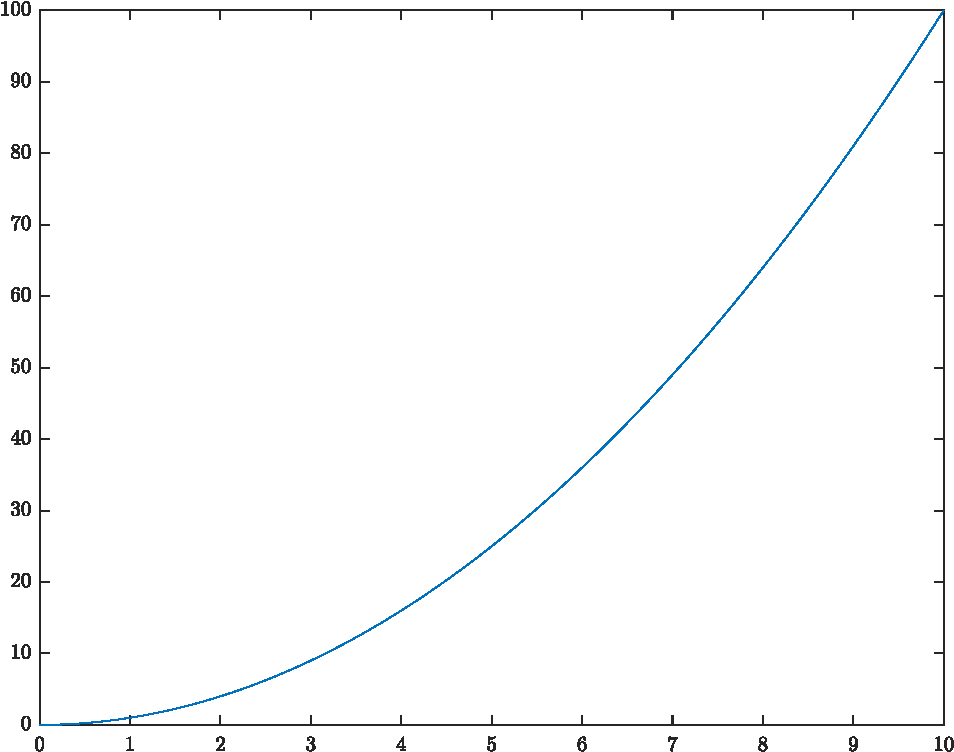
\includegraphics{gr-matlab.pdf}

This is the |misc/gr_matlab.m| input file:
\MyI{misc/gr_matlab.m}

I typed, on Linux,
\Shell{matlab -nodisplay -nodesktop -nosplash -r gr\_matlab}
in the |misc| subdirectory
to make the |graphics/gr-matlab.pdf| output file.
\end{VerbatimOut}

\MyIO


\begin{VerbatimOut}{z.out}

\section{\protect\METAPOSTLogo\ programming language}
\index{METAPOST@\METAPOSTLogo}  
\todoindex{\METAPOSTLogo}

\lightgreen{\MetaPostLogo\ uses \LaTeX\ fonts.}
\todoindex{\MetaPostLogo}

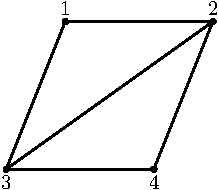
\includegraphics{gr-metapost-kim-1.pdf}
\hspace*{0.1truein}
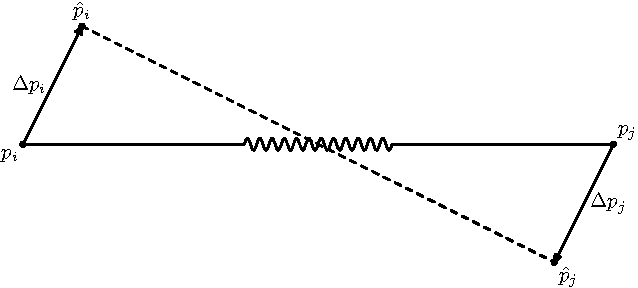
\includegraphics{gr-metapost-kim-2.pdf}

This is the |misc/gr-metapost-kim.mp| input file:
\MyI{misc/gr-metapost-kim.mp}

I typed, on Linux,\\
\hspace*{3\parindent}\Shell{mpost gr-metapost-kim}\\
\hspace*{3\parindent}\Shell{epstopdf gr-metapost-kim-1.mps;  epstopdf gr-metapost-kim-2.mps}\\
\hspace*{3\parindent}\Shell{mv -i gr-metapost-kim-1.pdf gr-metapost-kim-2.pdf ../graphics}\\
to run MetaPost and make two PDF files, |gr-metapost-kim-1.pdf| and |gr-metapost-kim-2.pdf|,
and move them to the graphics subfolder.
\end{VerbatimOut}

\MyIO


\begin{VerbatimOut}{z.out}

\subsection{Tally example}
\label{ss:tally-example}

Whenever I use files with numbers in them I like to put leading zeros
in the names so they will be listed in order in the directory.

These 20 graphics (|gr-metapost-tally-01.pdf| through |gr-metapost-tally-20.pdf|)

\vspace*{6pt}

{%
  % Let * represent zero or more spaces!
  % Method 1: \def\g#1{ requires using \g*{10} for 10.
  %           Two shifted characters, { and } are needed.
  % Method 2: \def\g#1/{ requires using \g*10/ for 10.
  %           One unshifted character, / is needed.
  \def\g#1/{\includegraphics[scale=0.5]{gr-metapost-tally-#1.pdf}}%

  % Note that tabular* instead of tabular is used below.
  %   The {\textwidth} makes the total width of the table the width
  % of the printed area of the page.
  %   The @{\kern2\parindent} puts blank space the width of two
  % paragraph indents before the first column.
  %   The @{extracolsep{\fill}} adds \fill space between all subsequent
  % columns.
  %   The lll left justifies the next three columns.
  % after the column.
  %   The @{\kern2\parindent} puts blank space the width of two
  % paragraph indents before the first column.
  \begin{tabular*}{\textwidth}{@{\kern2\parindent}@{\extracolsep{\fill}}lll@{\kern2\parindent}}%
    \g 01/& \g 02/& \g 03/\\
    \g 04/& \g 05/& \g 06/\\
    \g 07/& \g 08/& \g 09/\\
    \g 10/& \g 11/& \g 12/\\
    \g 13/& \g 14/& \g 15/\\
    \g 16/& \g 17/& \g 18/\\
    \g 19/& \g 20/\\
  \end{tabular*}%
}
\noindent were produced by

\MyI{misc/gr-metapost-tally.mp}

\end{VerbatimOut}

\MyIO


\begin{VerbatimOut}{z.out}
\section{Python programming language}
\ix{Python programming language}

\lightgreen{Python can be set up to use \LaTeX\ fonts.}

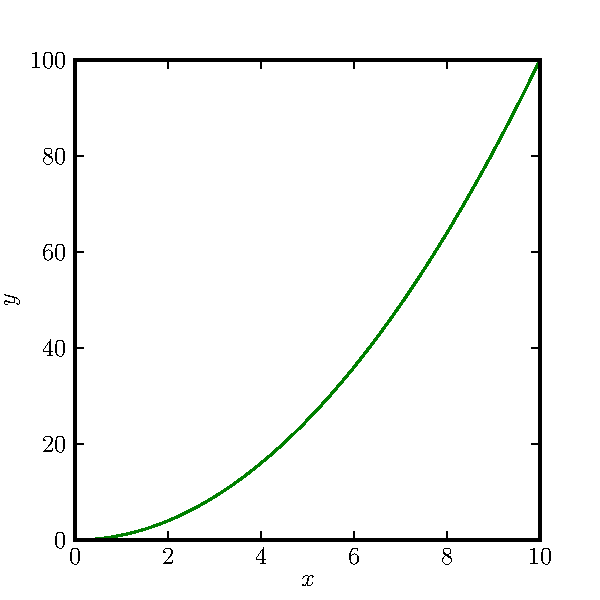
\includegraphics{gr-python2.pdf}

This is the |misc/gr-python2.py| input file:
\MyI{misc/gr-python2.py}

I typed, on Linux,
\Shell{./gr-python2.py}
in the |misc| subdirectory
to make the |graphics/gr-py|\\
|thon2.pdf| output file.
\end{VerbatimOut}

\MyIO



\begin{VerbatimOut}{z.out}

\section{R programming language}
\ix{R programming language}

\lightgreen{R can be set up to use \LaTeX\ fonts.}

% Created by tikzDevice version 0.6.2-92-0ad2792 on 2021-11-24 17:04:02
% !TEX encoding = UTF-8 Unicode
\begin{tikzpicture}[x=1pt,y=1pt]
\definecolor[named]{fillColor}{rgb}{1.00,1.00,1.00}
\path[use as bounding box,fill=fillColor,fill opacity=0.00] (0,0) rectangle (361.35,361.35);
\begin{scope}
\path[clip] ( 49.20, 61.20) rectangle (336.15,312.15);
\definecolor[named]{drawColor}{rgb}{0.00,0.00,0.00}

\path[draw=drawColor,line width= 0.4pt,line join=round,line cap=round] ( 59.83, 70.49) --
	( 62.48, 70.52) --
	( 65.14, 70.59) --
	( 67.80, 70.70) --
	( 70.46, 70.87) --
	( 73.11, 71.08) --
	( 75.77, 71.33) --
	( 78.43, 71.63) --
	( 81.08, 71.98) --
	( 83.74, 72.38) --
	( 86.40, 72.82) --
	( 89.05, 73.31) --
	( 91.71, 73.84) --
	( 94.37, 74.42) --
	( 97.03, 75.05) --
	( 99.68, 75.72) --
	(102.34, 76.44) --
	(105.00, 77.21) --
	(107.65, 78.02) --
	(110.31, 78.88) --
	(112.97, 79.79) --
	(115.62, 80.74) --
	(118.28, 81.74) --
	(120.94, 82.79) --
	(123.59, 83.88) --
	(126.25, 85.02) --
	(128.91, 86.20) --
	(131.57, 87.43) --
	(134.22, 88.71) --
	(136.88, 90.04) --
	(139.54, 91.41) --
	(142.19, 92.82) --
	(144.85, 94.29) --
	(147.51, 95.80) --
	(150.16, 97.36) --
	(152.82, 98.96) --
	(155.48,100.61) --
	(158.13,102.30) --
	(160.79,104.05) --
	(163.45,105.84) --
	(166.11,107.67) --
	(168.76,109.55) --
	(171.42,111.48) --
	(174.08,113.46) --
	(176.73,115.48) --
	(179.39,117.55) --
	(182.05,119.66) --
	(184.70,121.82) --
	(187.36,124.03) --
	(190.02,126.28) --
	(192.68,128.58) --
	(195.33,130.93) --
	(197.99,133.32) --
	(200.65,135.76) --
	(203.30,138.25) --
	(205.96,140.78) --
	(208.62,143.36) --
	(211.27,145.99) --
	(213.93,148.66) --
	(216.59,151.38) --
	(219.24,154.14) --
	(221.90,156.96) --
	(224.56,159.81) --
	(227.22,162.72) --
	(229.87,165.67) --
	(232.53,168.67) --
	(235.19,171.71) --
	(237.84,174.80) --
	(240.50,177.94) --
	(243.16,181.12) --
	(245.81,184.35) --
	(248.47,187.63) --
	(251.13,190.95) --
	(253.78,194.32) --
	(256.44,197.74) --
	(259.10,201.20) --
	(261.76,204.71) --
	(264.41,208.26) --
	(267.07,211.86) --
	(269.73,215.51) --
	(272.38,219.21) --
	(275.04,222.95) --
	(277.70,226.73) --
	(280.35,230.57) --
	(283.01,234.45) --
	(285.67,238.38) --
	(288.32,242.35) --
	(290.98,246.37) --
	(293.64,250.43) --
	(296.30,254.55) --
	(298.95,258.71) --
	(301.61,262.91) --
	(304.27,267.16) --
	(306.92,271.46) --
	(309.58,275.81) --
	(312.24,280.20) --
	(314.89,284.64) --
	(317.55,289.12) --
	(320.21,293.65) --
	(322.87,298.23) --
	(325.52,302.86);
\end{scope}
\begin{scope}
\path[clip] (  0.00,  0.00) rectangle (361.35,361.35);
\definecolor[named]{drawColor}{rgb}{0.00,0.00,0.00}

\path[draw=drawColor,line width= 0.4pt,line join=round,line cap=round] ( 59.83, 61.20) -- (325.52, 61.20);

\path[draw=drawColor,line width= 0.4pt,line join=round,line cap=round] ( 59.83, 61.20) -- ( 59.83, 55.20);

\path[draw=drawColor,line width= 0.4pt,line join=round,line cap=round] (112.97, 61.20) -- (112.97, 55.20);

\path[draw=drawColor,line width= 0.4pt,line join=round,line cap=round] (166.11, 61.20) -- (166.11, 55.20);

\path[draw=drawColor,line width= 0.4pt,line join=round,line cap=round] (219.24, 61.20) -- (219.24, 55.20);

\path[draw=drawColor,line width= 0.4pt,line join=round,line cap=round] (272.38, 61.20) -- (272.38, 55.20);

\path[draw=drawColor,line width= 0.4pt,line join=round,line cap=round] (325.52, 61.20) -- (325.52, 55.20);

\node[text=drawColor,anchor=base,inner sep=0pt, outer sep=0pt, scale=  1.00] at ( 59.83, 39.60) {0};

\node[text=drawColor,anchor=base,inner sep=0pt, outer sep=0pt, scale=  1.00] at (112.97, 39.60) {2};

\node[text=drawColor,anchor=base,inner sep=0pt, outer sep=0pt, scale=  1.00] at (166.11, 39.60) {4};

\node[text=drawColor,anchor=base,inner sep=0pt, outer sep=0pt, scale=  1.00] at (219.24, 39.60) {6};

\node[text=drawColor,anchor=base,inner sep=0pt, outer sep=0pt, scale=  1.00] at (272.38, 39.60) {8};

\node[text=drawColor,anchor=base,inner sep=0pt, outer sep=0pt, scale=  1.00] at (325.52, 39.60) {10};

\path[draw=drawColor,line width= 0.4pt,line join=round,line cap=round] ( 49.20, 70.49) -- ( 49.20,302.86);

\path[draw=drawColor,line width= 0.4pt,line join=round,line cap=round] ( 49.20, 70.49) -- ( 43.20, 70.49);

\path[draw=drawColor,line width= 0.4pt,line join=round,line cap=round] ( 49.20,116.97) -- ( 43.20,116.97);

\path[draw=drawColor,line width= 0.4pt,line join=round,line cap=round] ( 49.20,163.44) -- ( 43.20,163.44);

\path[draw=drawColor,line width= 0.4pt,line join=round,line cap=round] ( 49.20,209.91) -- ( 43.20,209.91);

\path[draw=drawColor,line width= 0.4pt,line join=round,line cap=round] ( 49.20,256.38) -- ( 43.20,256.38);

\path[draw=drawColor,line width= 0.4pt,line join=round,line cap=round] ( 49.20,302.86) -- ( 43.20,302.86);

\node[text=drawColor,rotate= 90.00,anchor=base,inner sep=0pt, outer sep=0pt, scale=  1.00] at ( 34.80, 70.49) {0};

\node[text=drawColor,rotate= 90.00,anchor=base,inner sep=0pt, outer sep=0pt, scale=  1.00] at ( 34.80,116.97) {20};

\node[text=drawColor,rotate= 90.00,anchor=base,inner sep=0pt, outer sep=0pt, scale=  1.00] at ( 34.80,163.44) {40};

\node[text=drawColor,rotate= 90.00,anchor=base,inner sep=0pt, outer sep=0pt, scale=  1.00] at ( 34.80,209.91) {60};

\node[text=drawColor,rotate= 90.00,anchor=base,inner sep=0pt, outer sep=0pt, scale=  1.00] at ( 34.80,256.38) {80};

\node[text=drawColor,rotate= 90.00,anchor=base,inner sep=0pt, outer sep=0pt, scale=  1.00] at ( 34.80,302.86) {100};

\path[draw=drawColor,line width= 0.4pt,line join=round,line cap=round] ( 49.20, 61.20) --
	(336.15, 61.20) --
	(336.15,312.15) --
	( 49.20,312.15) --
	( 49.20, 61.20);
\end{scope}
\begin{scope}
\path[clip] (  0.00,  0.00) rectangle (361.35,361.35);
\definecolor[named]{drawColor}{rgb}{0.00,0.00,0.00}

\node[text=drawColor,anchor=base,inner sep=0pt, outer sep=0pt, scale=  1.00] at (192.68, 15.60) {$x$};

\node[text=drawColor,rotate= 90.00,anchor=base,inner sep=0pt, outer sep=0pt, scale=  1.00] at ( 10.80,186.67) {$y$};
\end{scope}
\end{tikzpicture}


This is the |misc/gr-r.R| input file:
\MyI{misc/gr-r.R}

I typed, on Linux,
\Shell{R CMD BATCH gr-r}
in the |misc| subdirectory to make the |gr-r.tex| outfile file.
\end{VerbatimOut}

\MyIO


\begin{VerbatimOut}{z.out}

\section{\TikZLogo\ \LaTeX\ package}
\index{TikZ@\TikZLogo\ \LaTeX\ package}  
\todoindex{\TikZLogo\ \LaTeX\ package}

\lightgreen{\TikZLogo\ uses \LaTeX\ fonts.}
\end{VerbatimOut}

\MyIO


\begin{VerbatimOut}{z.out}

\subsection{Clock example}
\index{clock \TikZLogo\ example}
\todoindex{clock \TikZLogo\ example}
\end{VerbatimOut}

\MyIO


\begin{VerbatimOut}{z.out}

\index{TikZ@\TikZLogo}

\hbox to\textwidth{%
  \hfil
  % The idea for this clock was originally from a Google+ posting by Afamefuna ``Ferdy'' Ibeabuchia.
  \begin{tikzpicture}
    \def\CenterRadius{0.04cm}
    \def\InnerTickRadius{3.6cm}
    \def\OuterTickRadius{3.8cm}
    % Make \LR be an abbreviation for \LabelRadius so the
    % lines below will fit within the width of the page.
    \def\LabelRadius{4.5cm}      \let\LR=\LabelRadius
    \def\HourHandRadius{2.5cm}   \def\HourHandBase{0.3cm}
    \def\MinuteHandRadius{3cm}   \def\MinuteHandBase{0.4cm}
    \def\SecondHandRadius{3.5cm} \def\SecondHandBase{0.5cm}
    \def\DS{\displaystyle}
    \fill (0,0) circle (\CenterRadius);
    \foreach \i in {0,30,...,330}
    \draw (\i:\InnerTickRadius)--(\i:\OuterTickRadius);
    \node at (  0:\LR) {$\DS \qquad \sqrt9 + 9 - 9$};        %  3
    \node at ( 30:\LR) {$\DS \frac{9+9}9$};                  %  2
    \node at ( 60:\LR) {$\DS \frac{\sqrt9\sqrt9}9$};         %  1
    \node at ( 90:\LR) {$\DS 9 + \frac9{\sqrt9}$};           % 12
    \node at (120:\LR) {$\DS \frac{99}9$};                   % 11
    \node at (150:\LR) {$\DS 9 + \frac99$};                  % 10
    \node at (180:\LR) {$\DS \sqrt[\scriptstyle 9]{9^9}$};   %  9
    \node at (210:\LR) {$\DS 9 - \frac99$};                  %  8
    \node at (240:\LR) {$\DS 9 - \sqrt9 + \lceil.9\rceil$};  %  7
    \node at (270:\LR) {$\DS 9 - \frac9{\sqrt9}$};           %  6
    \node at (300:\LR) {$\DS \sqrt9\,! - \frac99$};          %  5
    \node at (330:\LR) {$\DS \sqrt9 + \frac99$};             %  4
    % In the following
    %   ABBREVIATION    DESCRIPTION
    %   deg             degrees
    %   min             minutes
    %   sec             seconds
    % for second hand:
    %   (9 sec/60 sec) * 360 deg = 54 deg;
    %   90 deg - 54 deg = 36 deg
    \draw[rotate around={36:(0,0)}]
      (-\SecondHandBase,\SecondHandBase) -- (\SecondHandRadius,0)
        -- (-\SecondHandBase,-\SecondHandBase) -- cycle;
    % for minute hand:
    %   (9 min/60 min) * 360 deg = 54 deg;
    %   90 deg - 54 deg = 36 deg
   \draw[rotate around={36:(0,0)}]
     (-\MinuteHandBase,\MinuteHandBase) -- (\MinuteHandRadius,0)
       -- (-\MinuteHandBase,-\MinuteHandBase) -- cycle;
    % for hour hand:
    %   (9 min * (60 sec/1 min)) + 9 sec) / 3600 sec
    %     = 549 sec / 3600 sec = 0.1525
    %   The hour hand is 0.1525 of the way from 9:00 to 10:00.
    %   Each hour is 30 degrees on the clock, so the hour hand
    %   position is
    %     30 deg * 0.1525 = 4.575 deg past 9:00
    %   180 deg - 4.575 deg = 175.425 deg
    \draw[rotate around={175.425:(0,0)}]
      (-\HourHandBase,\HourHandBase) -- (\HourHandRadius,0)
      -- (-\HourHandBase,-\HourHandBase) -- cycle;
  \end{tikzpicture}
  \hfil
}
\end{VerbatimOut}

\MyIO


\begin{VerbatimOut}{z.out}

\newpage

\subsection{Counter example}
\index{Counter \TikZLogo\ example}
\todoindex{Counter \TikZLogo\ example}

\begin{tikzpicture}[scale=0.13]
  % Define points.
  \coordinate   (p11) at (  0, 78);
    \coordinate (p14) at ( 35, 78);
    \coordinate (p15) at ( 54, 78);
    \coordinate (p16) at ( 73, 78);
    \coordinate (p19) at (108, 78);
  \coordinate   (p24) at ( 35, 67);
    \coordinate (p26) at ( 73, 67);
  \coordinate   (p35) at ( 54, 63);
  \coordinate   (p44) at ( 35, 56);
    \coordinate (p46) at ( 73, 56);
  \coordinate   (p53) at ( 30, 48);
    \coordinate (p55) at ( 54, 48);
    \coordinate (p57) at ( 78, 48);
  \coordinate   (p69) at (108, 39);
  \coordinate   (p71) at (  0, 24);
    \coordinate (p72) at ( 15, 24);
    \coordinate (p73) at ( 30, 24);
    \coordinate (p75) at ( 54, 24);
    \coordinate (p77) at ( 78, 24);
    \coordinate (p78) at ( 93, 24);
    \coordinate (p79) at (108, 24);
  \coordinate   (p81) at (  0,  0);
    \coordinate (p83) at ( 30,  0);
    \coordinate (p85) at ( 54,  0);
    \coordinate (p87) at ( 78,  0);
    \coordinate (p89) at (108,  0);
  % Put "wall" above drawing.
  \draw (p15) node[above] {\large wall};
  % Plot outer edge.
  \draw (p81) -- (p11) -- (p19) -- (p89);
  % Plot inner edge.
  \draw (p83) -- (p53) -- (p57) -- (p87);
  % Color the counter. 
  \fill[blue!10] (p81) -- (p11) -- (p19) -- (p89) -- (p87) -- (p57) -- (p53) -- (p83) -- cycle;
  % Vertical measurement lines.
  \draw[dashed, arrows = {Stealth[inset=0pt, angle=30:8pt]-Stealth[inset=0pt, angle=30:8pt]}]
    (p14) -- (p44);
  \draw (p24) node[fill=blue!10] {$22''$};
  \draw[arrows = {Stealth[inset=0pt, angle=30:8pt]-Stealth[inset=0pt, angle=30:8pt]}] (p15) -- (p55);
  \draw (p35) node[fill=blue!10] {$30''$};
  \draw[dashed, arrows = {Stealth[inset=0pt, angle=30:8pt]-Stealth[inset=0pt, angle=30:8pt]}]
    (p16) -- (p46);
  \draw (p26) node[fill=blue!10] {$22''$};
  \draw[arrows = {Stealth[inset=0pt, angle=30:8pt]-Stealth[inset=0pt, angle=30:8pt]}] (p55) -- (p85);
  % Horizontal measurement lines.
  \draw[arrows = {Stealth[inset=0pt, angle=30:8pt]-Stealth[inset=0pt, angle=30:8pt]}] (p71) -- (p73);
  \draw (p72) node[fill=blue!10] {$30''$};
  \draw[arrows = {Stealth[inset=0pt, angle=30:8pt]-Stealth[inset=0pt, angle=30:8pt]}] (p73) -- (p77);
  \draw (p75) node[fill=white] {$48''$};
  \draw[arrows = {Stealth[inset=0pt, angle=30:8pt]-Stealth[inset=0pt, angle=30:8pt]}] (p77) -- (p79);
  \draw (p78) node[fill=blue!10] {$30''$};
  % Put "wall" to the right of drawing.
  \draw (p69) node[right] {\large wall};
\end{tikzpicture}
\end{VerbatimOut}

\MyIO


\begin{VerbatimOut}{z.out}

\subsection{Fourier transform example}
\index{Fourier transform \TikZLogo\ example}
\todoindex{Fourier transform \TikZLogo\ example}
  
The Fourier transform decomposes a function
into the frequencies that make it up.
The inverse Fourier transformation combines the contributions
of all the different frequencies to recover the original function.

(Mark Senn {\tt\char'074}mark@purdue.edu{\tt\char'076} wrote sales@aavos.be on 2021-09-03
to ask permission
to use
\href{https://aavos.eu/glossary/fourier-transform/}{Fourier transform}
as the starting point
for an example \TikZLogo\ figure.  
Dominique Demurie {\tt\char'074}sales@aavos.be{\tt\char'076} replied
on 2021-09-06 with
``I think it is not an original drawing from us either.
We had it for years on our website,
but I cannot remember where we got it from.
We don't mind you using it for a thesis.'')

% Run this with
%     pdflatex --shell-escape t
% That makes the t.table.* files.
%
% See
%     https://ctan.math.washington.edu/tex-archive/graphics/pgf/base/doc/pgfmanual.pdf
%     PAGE    TOPIC
%      655    decorations.text library to draw text 
%     1221    animations
%
% for text decorations, which includes text along a path information.
% Also see
%     https://tex.stackexchange.com/questions/427454/tikz-3dplot-and-rotation-of-coordinates
%     https://tex.stackexchange.com/questions/67573/tikz-shift-and-rotate-in-3d
%     http://tug.ctan.org/graphics/pgf/contrib/tikz-3dplot/tikz-3dplot_documentation.pdf
%     https://tex.stackexchange.com/questions/45848/rotate-node-text-and-use-relative-positioning-in-tikz
  
% was scale = 2
\begin{tikzpicture}[domain=0:6.283185, rotate around y=-55, scale=1]

  % total plot
  \begin{scope}[canvas is xy plane at z=0]
    \node[below=3pt] at (0,        -1) {0};
    \node[below=3pt] at (3.141593, -1) {$\pi$};
    \node[below=5pt] at (5.683185, -1) {$2\pi$};
    \draw[ultra thick,color=violet] plot[id=total,smooth] function{0.8*sin(x)+0.2*sin(8*x)};
    \draw[thin,color=black] (0,-1) -- (0,1) -- (6.283185,1) -- (6.283185,-1) -- cycle;
    \draw[thin,color=black] (0,0) -- (6.283185,0);
    \path[decorate,decoration={text along path,
% |\LARGE|
      text={Time Domain}}] (0.1,-2) -- (6.283185,-2); 
    % $s(t)$
  \end{scope}

  % tall plot
  \begin{scope}[canvas is xy plane at z=-1.5]
    \draw[dashed] (0,0.8) -- (6.283185,0.8);
    \draw[dashed] (0,-0.8) -- (6.283185,-0.8);
    \draw[thick,color=orange] plot[id=tall,smooth] function{0.8*sin(x)};
    \draw[thin,color=black] (0,-1) -- (0,1) -- (6.283185,1) -- (6.283185,-1) -- cycle;
    \draw[thin,color=black] (0,0) -- (6.283185,0);
  \end{scope}

  % short plot
  \begin{scope}[canvas is xy plane at z=-3.0]
    \draw[dashed] (0, 0.2) -- (6.283185,  0.2);
    \draw[dashed] (0,-0.2) -- (6.283185, -0.2);
    \draw[thick,color=green] plot[id=short,smooth] function{0.2*sin(2*x)};
    \draw[thin,color=black] (0,-1) -- (0,1) -- (6.283185,1) -- (6.283185,-1) -- cycle;
    \draw[thin,color=black] (0,0) -- (6.283185,0);
  \end{scope}

  % frequency plot
  \begin{scope}[canvas is zy plane at x=6.283185]
    \node[below=3pt] at ( 0.0,-1) {0};
    \node[below=3pt] at (-1.5,-1) {1};
    \node[below=3pt] at (-3.0,-1) {2};
    \draw[thin,color=black] (0,-1.0) -- (-3.0,-1.0);  \node[above=-9pt] at (-3.3,-1.0) {$-1.0$};
    \draw[thin,color=black] (0,-0.8) -- (-3.0,-0.8);  \node[above=-9pt] at (-3.3,-0.8) {$-0.8$};
    \draw[thin,color=black] (0,-0.2) -- (-3.0,-0.2);  \node[above=-9pt] at (-3.3,-0.2) {$-0.2$};
    \draw[thin,color=black] (0, 0.0) -- (-3.0, 0.0);  \node[above=-9pt] at (-3.3, 0.0) {$\phantom{-}0.0$};
    \draw[thin,color=black] (0, 0.2) -- (-3.0, 0.2);  \node[above=-9pt] at (-3.3, 0.2) {$\phantom{-}0.2$};
    \draw[thin,color=black] (0, 0.8) -- (-3.0, 0.8);  \node[above=-9pt] at (-3.3, 0.8) {$\phantom{-}0.8$};
    \draw[thin,color=black] (0, 1.0) -- (-3.0, 1.0);  \node[above=-9pt] at (-3.3, 1.0) {$\phantom{-}1.0$};
    \draw[line width=6pt,color=red] (-1.5,0) -- (-1.5,0.8);
    \draw[line width=6pt,color=red] (-3.0,0) -- (-3.0,0.2);
    \path[decorate,decoration={text along path,
% |\LARGE|
      text={Frequency Domain}}] (-0.8,-1.6) -- (-3.0,-1.6); 
    % $S(\omega)$
  \end{scope}

  %% legend
  %% Wolfram Language code:
  %%     In[1]:= ry[theta_] :=
  %%     {
  %%         {Cos[theta Degree],  0, Sin[theta Degree]},
  %%         {0,                  1, 0},
  %%         {-Sin[theta Degree], 0, Cos[theta Degree]}
  %%     }
  %%
  %%     ry[55] . {Pi, 0.7, -3.5}
  %%     # Out[] = {-1.06509, 0.7, -4.58096}
  %%     ry[55] . {(3/4)Pi, 0.7, -3.5}
  %%     # Out[] = {-1.51557, 0.7, -3.9376}

  \draw[ultra thick,color=violet] (2.45782, 1.7, -4.33538) -- (1.06509, 0.7, -4.58096);
    \node[right] at                                            (1.06509, 0.7, -4.58096) {$0.8\sin x + 0.2\sin 2x$};
  \draw[ultra thick,color=orange] ( 0.08509, 0.4, -4.58096) -- (1.06509, 0.4, -4.58096);
    \node[right] at                                            (1.06509, 0.4, -4.58096) {$0.8\sin x$};
  \draw[ultra thick,color=green]  ( 0.08509, 0.1, -4.58096) -- (1.06509, 0.1, -4.58096);
    \node[right] at                                            (1.06509, 0.1, -4.58096) {$0.2\sin 2x$};
\end{tikzpicture}
\end{VerbatimOut}

\MyIO


\begin{VerbatimOut}{z.out}

\subsection{Glider example}
\ix{Hirzel, Alex}
\index{glider \TikZLogo\ example}
\todoindex{glider \TikZLogo\ example}

The glider
is a pattern from the Game of Life,
and it's used as an emblem representing the hacker community.

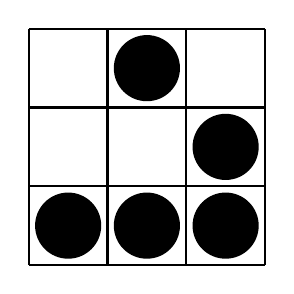
\begin{tikzpicture}[thick]
  \draw (0,0) grid (3,3);
  \foreach \c in {(0,0), (1,0), (2,0), (2,1), (1,2)}
    \fill \c + (0.5,0.5) circle (0.42);
\end{tikzpicture}
\end{VerbatimOut}

\MyIO


\begin{VerbatimOut}{z.out}

\newpage

\subsection{Tree example}
\ix{???, ???}
\index{tree \TikZLogo\ example}
\todoindex{tree \TikZLogo\ example}

{
  \def\f#1#2{$\displaystyle\frac #1#2$}
  \begin{tikzpicture}%
  [%
    level 1/.style={sibling distance=60mm},
    level 2/.style={sibling distance=30mm},
    level 3/.style={sibling distance=15mm}
  ]
    \node {\f 11}
      child {node {$\displaystyle\frac 12$}
        child {node {\f 13}
          child {node {\f 14}}
          child {node {\f 48}}
        }
        child {node {\f 32}
          child {node {\f 35}}
          child {node {\f 52}}
        }
      }
      child {node {\f 21}
        child {node {\f 23}
          child {node {\f 25}}
          child {node {\f 53}}
        }
        child {node {\f 31}
          child {node {\f 34}}
          child {node {\f 41}}
        }
      };
  \end{tikzpicture}    

\vspace*{4pt}
The node with value \f nd\\[2pt]
\indent\hspace*{4\parindent}
\begin{tabular}{@{}llll@{}}
  \bfseries with additional conditions& \bfseries has& \bfseries with value\\
  \noalign{\vspace{2pt}}
  (none)&                     left child&     \f n{{n+d}}\\
  \noalign{\vspace{12pt}}
  (none)&                     right child&    \f {{n+d}}d\\
  \noalign{\vspace{12pt}}
  $n<d$&                      parent&         \f n{{d-n}}\\
  \noalign{\vspace{12pt}}
  $n=d$&                      no parent&      (not applicable)\\
  \noalign{\vspace{12pt}}
  $n>d$&                      parent&         \f {{n-d}}d\\
\end{tabular}
}
\end{VerbatimOut}

\MyIO

\begin{VerbatimOut}{z.out}


\subsection{Yin and yang example}

This Yin and yang example was done by Thomas G. Kristensen \cite{kristensen}.
This is the ``traditional Taijitu symbol from Chinese philosophy''.
\ix{Kristensen, Thomas G.//Taijitu symbol//Yin and yang symbol}

\index{TikZ@\TikZLogo}  

\begin{tikzpicture}
  % Yin and yang
  % Author: Thomas G. Kristensen
  
  % color one half of a unit circle                                              
  \begin{scope}
    \clip (0,0) circle (1cm);
    \fill[black] (0cm,1cm) rectangle (-1cm, -1cm);
  \end{scope}

  % fill heads                                                                   
  \fill[black] (0,0.5) circle (0.5cm);
  \fill[white] (0,-0.5) circle (0.5cm);

  % fill eyes                                                                    
  \fill[white] (0,0.5) circle (0.1cm);
  \fill[black] (0,-0.5) circle (0.1cm);

  % outer line                                                                   
  \draw (0,0) circle (1cm);

\end{tikzpicture}
\end{VerbatimOut}

\MyIO


\begin{VerbatimOut}{z.out}

\section{Wolfram Language (Mathematica uses this)}
\ix{Mathematica}
\ix{Wolfram Language}

\lightgreen{Wolfram Language can be set up to use \LaTeX\ fonts.}

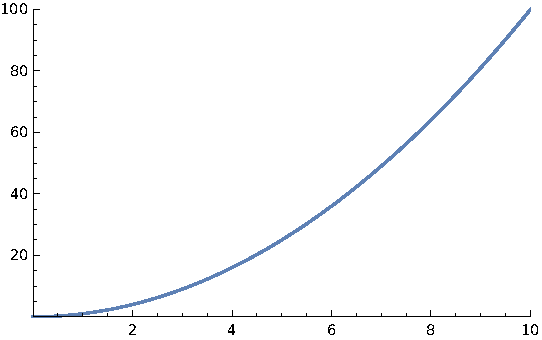
\includegraphics{gr-mathematica.pdf}

This is the |misc/gr-mathematica.ma| input file
\MyI{misc/gr-mathematica.ma}

I typed, on Linux,
\Shell{math < gr-mathematica.ma}
in the |misc| subdirectory
to make the |graphics/gr-mathematica.pdf| output file.
\end{VerbatimOut}

\MyIO
